\documentclass[12pt,a4paper]{article}
\usepackage[utf8]{inputenc}
\usepackage[T1]{fontenc}
\usepackage{lmodern}
\usepackage[margin=2.5cm]{geometry}
\usepackage{amsmath,amssymb,amsthm}
\usepackage{booktabs}
\usepackage{graphicx}
\usepackage{xcolor}
\usepackage[colorlinks=true,linkcolor=blue!50!black,citecolor=blue!50!black,urlcolor=blue!50!black]{hyperref}

\newcommand{\vol}{\operatorname{vol}}
\newcommand{\U}{\mathcal{U}}
\newcommand{\R}{\mathbb{R}}
\newcommand{\Pfree}{\Phi_{\mathrm{free}}}
\newcommand{\Pcomp}{\Phi_{\mathrm{comp}}}
\newcommand{\Psic}{\Psi_{\mathrm{comp}}}
\newcommand{\code}[1]{\texttt{#1}}
\newtheorem{observation}{Observation}
\makeatletter\newcommand{\tabinput}[1]{\@@input #1.tex }\makeatother

\title{An Implementation of the $n^{O(\sqrt{k})}$ Algorithm for\\
3-D Hypervolume Subset Selection\\[0.5ex]
\large Technical report accompanying the \code{hssp3d} Python/Numba package}
\author{Michael Emmerich\\[0.5ex]
\normalsize University of Jyv\"askyl\"a}
\date{\today}

\begin{document}
\maketitle

\begin{abstract}
\noindent
The hypervolume subset selection problem (HSSP) asks for $k$ out of $n$ points that
maximise the hypervolume indicator.  In three dimensions the problem is NP-hard, and
Bringmann, Cabello and Emmerich~\cite{BCE} gave the first exact algorithm that avoids
the enumeration of all $\binom{n}{k}$ subsets: a dynamic programme over planar separators
of the projected optimal solution with running time $n^{O(\sqrt{k})}$.  This report
describes a complete implementation of that algorithm in Python with Numba-compiled
kernels~\cite{Numba}, states precisely where and why it deviates from the description in the paper,
and validates it against brute-force enumeration on random samples of the DTLZ1 and DTLZ2
Pareto fronts with $15$ points.  The dynamic programme reproduced the brute-force optimum
on every instance.  As expected for an algorithm whose merit is asymptotic, it is orders of
magnitude slower than enumeration for inputs of this size; the role of the constants hidden
in the $O(\sqrt{k})$ is discussed and measured.
\end{abstract}

\section{Problem}
For $p\in\R^3_{>0}$ let $\mathrm{box}(p)=[0,p_1]\times[0,p_2]\times[0,p_3]$, for a finite
set $Q$ let $\U(Q)=\bigcup_{q\in Q}\mathrm{box}(q)$ and $\mu(Q)=\vol(\U(Q))$.  Given a set
$P$ of $n$ points and $k\le n$, \textsc{Volume Selection} asks for
\[
  \mathrm{VolSel}(P,k)=\max_{S\subseteq P,\;|S|=k}\mu(S)
\]
together with a maximiser.  For a minimisation problem with objective vectors $f$ and
reference point $r$, the substitution $p=r-f$ turns the hypervolume indicator into $\mu$;
the package accepts both conventions.  Dominated points never need to be selected and are
removed beforehand, and ties in a coordinate are broken by the perturbation
$p+i\varepsilon(1,1,1)$ suggested in~\cite{BCE}, so that $P$ is an antichain in general
position.

\section{The algorithm of Bringmann, Cabello and Emmerich}
\label{sec:alg}
We recall the construction of \cite[Section~4]{BCE} in the form in which it is implemented.

\paragraph{Projection graph and triangulation.}
The boundary of $\U(Q)$, projected onto the $xy$-plane, is a plane graph $G(Q)$ with
vertices $v_q$ (the corner of $q$), $v_{q,q'}$ (a T-junction of two box boundaries),
$v_{x,q},v_{y,q}$ (on the axes) and the origin.  Every bounded face $f(q,Q)$ is the part
of the plane on which $q$ is the highest box; it is bounded by a top segment, a right
segment and a monotone staircase $\gamma(q,Q)$.  The \emph{canonical triangulation}
adds diagonals from $v_q$ to the interior vertices of $\gamma(q,Q)$, from the first interior
vertex of $\gamma$ to the vertices of the top segment and from the last one to those of the
right segment.  The outer face is triangulated towards the corners of a square
$\sigma\supset G(Q)$.  The result $T(Q)$ is a triangulation of $\sigma$ with $O(|Q|)$
vertices.  A polygonal domain $D$ is \emph{$Q$-compliant} if its boundary consists of edges
of $T(Q)$, and $P_\gamma$ denotes the points that define the vertices of a curve $\gamma$.

\paragraph{Subproblems.}
A valid tuple $(S,D,\ell)$ consists of the points $S$ selected so far, an $S$-compliant
domain $D$, and a budget $\ell$ of points that may still be chosen in $P\cap(D\times\R)$:
\begin{align*}
 \Pfree(S,D,\ell) &=\max\{\vol(\U(S\cup Q)\cap(D\times\R)) : Q\subseteq P\cap(D\times\R),\ |Q|\le\ell\},\\
 \Pcomp(S,D,\ell) &=\text{the same maximum over those $Q$ for which $D$ is $(S\cup Q)$-compliant.}
\end{align*}
A \emph{valid partition} of $(S,D,\ell)$ is a family $\{(S\cup S_0,D_i,\ell_i)\}_i$ with
$S_0\subseteq P\cap D$, $|S_0|=O(\sqrt{|S|+\ell})$, $(S\cup S_0)$-compliant domains $D_i$
with disjoint interiors and union $D$, $\ell=|S_0|+\sum_i\ell_i$ and $\ell_i\le 2\ell/3$.
The algorithm evaluates
\begin{equation}\label{eq:psi}
 \Psic(S,D,\ell)=
 \begin{cases}
   \Pcomp(S,D,\ell) & \text{if }\ell\le O(\sqrt{k}),\\[0.5ex]
   \displaystyle\max_{\pi\in\Pi(S,D,\ell)}\ \sum_{(S',D',\ell')\in\pi}\Psic(S',D',\ell') & \text{otherwise.}
 \end{cases}
\end{equation}

\paragraph{Correctness and running time.}
Every valid partition glues feasible solutions of its parts into a feasible solution of the
whole (Lemma~4.3), so $\Psic\le\Pfree$.  Conversely, for the optimal $Q^*$ of
$\Pcomp(S,D,\ell)$, Miller's theorem~\cite{Miller} yields a simple cycle $\gamma$ in
$T(S\cup Q^*)$ with $O(\sqrt{|S|+\ell})$ vertices that has at most $2|Q^*|/3$ of the
vertices $v_q$, $q\in Q^*$, on either side; $S_0=P_\gamma\setminus S$ and the pieces into
which $\gamma$ cuts $D$ form a valid partition whose value is at least
$\Pcomp(S,D,\ell)$ (Lemma~4.4).  Hence
$\Pcomp\le\Psic\le\Pfree$ (Lemma~4.5), and since
$\Pcomp(\emptyset,\sigma,k)=\Pfree(\emptyset,\sigma,k)=\mathrm{VolSel}(P,k)$ the top-level
value is optimal.  Along any chain of the recursion $|S|=O(\sqrt{k})$, which bounds the
number of tuples and the work per tuple by $n^{O(\sqrt{k})}$ (Theorem~4.6).

\section{Implementation}
The package \code{hssp3d} consists of Numba-compiled kernels (\code{\_kernels.py}) for all
geometric and combinatorial inner loops and a memoised Python recursion over the valid tuples
(\code{solver.py}).

\paragraph{A common vertex space.}
Compliance compares edges of \emph{different} triangulations $T(Q)$ and $T(Q')$.  Every vertex
of every $T(Q)$, $Q\subseteq P$, has the $x$-coordinate of some point (or $0$, or a side of
$\sigma$) and likewise for $y$.  Vertices are therefore identified by their pair of coordinate
\emph{ranks}, a global integer id on an $(n+3)\times(n+3)$ grid.  Edges and triangles of different
triangulations become directly comparable, and the set $P_v$ of points defining a vertex can be
read off its id.  Geometry (areas, orientation, point location) uses the real coordinates.

\paragraph{The triangulation $T(Q)$.}
\code{build\_T} processes the points by decreasing $z$.  For a point $q$ the start of the
visible part of its top edge is $\max\{a_x: a_z>q_z,\ a_y>q_y\}$ (or the $y$-axis), analogously
for the right edge; the staircase $\gamma(q,Q)$ is traced through the two-dimensional skyline
of the higher boxes, including the pieces that run along the axes; the T-junctions on the top
(right) segment of $q$ are the lower boxes whose right (top) edge ends there.  The fans
described in Section~\ref{sec:alg} are emitted as counter-clockwise triangles, each labelled with the
point $q$ owning the face.  The cost is $O(|Q|^2)$.  Inside a triangle of $T(Q)$ the height of
$\U(Q)$ is constant, hence for every $Q$-compliant domain $D$
\[
  \vol\bigl(\U(Q)\cap(D\times\R)\bigr)=\sum_{t\in T(Q),\,t\subseteq D}\mathrm{area}(t)\cdot z_{\mathrm{owner}(t)} .
\]
Figure~\ref{fig:T} shows an example.
The unit tests verify for all subsets of several point sets that the output has $2|V|-6$
triangles (Euler's formula for a triangulated square), that all triangles have positive area
summing to the area of $\sigma$, that every interior edge is shared by exactly two triangles
with opposite orientation, and that the formula above with $D=\sigma$ equals the exact
hypervolume computed by an independent sweep (which in turn is tested against
inclusion--exclusion).

\begin{figure}[t]
\centering
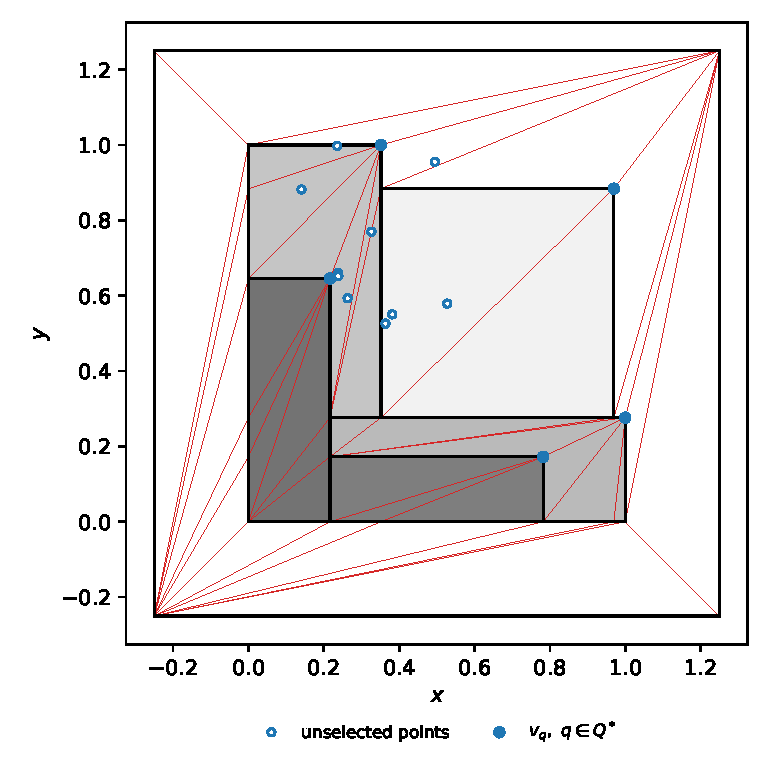
\includegraphics[width=0.62\textwidth]{fig_triangulation}
\caption{The triangulation $T(Q^*)$ computed by \code{build\_T} for the optimal $5$-subset $Q^*$ of a
DTLZ2 instance with $n=15$ (seed $0$, $k=5$ in Table~\ref{tab:values}), in normalised anchored-box
coordinates $p=r-f$.  Black: the projection graph
$G(Q^*)$; red: diagonals of the canonical triangulation and of the outer face; faces are shaded by the height
$z_q$ of their box (darker is higher).  A separator is a short cycle in this graph.}
\label{fig:T}
\end{figure}

\paragraph{Compliance test and restricted volume.}
A domain is stored as the set of triangles of $T(S)$ it consists of (a bit mask, which together
with $S$ and $\ell$ forms the memoisation key) and handed to other triangulations as the list of
its directed boundary edges, with $D$ on the left.  \code{eval\_in\_domain} enters the directed
edges of $T(S\cup Q)$ into a stamped table, checks that every boundary edge of $D$ is present
(this is exactly $(S\cup Q)$-compliance), and flood-fills the triangles of $T(S\cup Q)$ inside
$D$ starting from the triangles to the left of the boundary edges.  One evaluation costs
$O(|S\cup Q|^2)$, dominated by \code{build\_T}.

\paragraph{Base case.}
\code{base\_case} is Lemma~4.2 verbatim: all $Q\subseteq P\cap D$ with $|Q|\le\ell$ are
enumerated, non-compliant ones are discarded, and the restricted volume is maximised.

\paragraph{Valid partitions.}
Following the remark in the proof of Theorem~4.6, partitions are generated from cycles rather
than from arbitrary edge subsets.  For every $S_0\subseteq P\cap D$ with
$|S_0|\le\lceil c_{s}\sqrt{|S|+\ell}\,\rceil$ the triangulation $T(S\cup S_0)$ is built; if $D$ is
not $(S\cup S_0)$-compliant, $S_0$ is discarded (by Lemma~4.1 this cannot happen for the
separator of the optimal solution).  Then all simple cycles $\gamma$ of $T(S\cup S_0)$ with
$|\gamma|\le\lceil c_{\gamma}\sqrt{|S|+\ell}\,\rceil$ and $P_\gamma\setminus S=S_0$ that cut $D$
are enumerated by a depth-first search.  Since the domains of all tuples are connected, a cycle cuts $D$ if
and only if it uses an edge interior to $D$; each
cycle is generated exactly once, from its lowest-ranked interior edge.  The search is pruned by
the breadth-first distance back to the start vertex and by the number of points of $S_0$ that
still have to be covered (a vertex is defined by at most two points).  Distinct cycles that
induce the same subdivision of $D$ are merged.  The connected components of the two sides are
the domains $D_i$; components without candidate points contribute the constant
$\vol(\U(S\cup S_0)\cap(D_i\times\R))$, and the budgets $\ell_i\le\lfloor 2\ell/3\rfloor$ of the
others are optimised by a max-plus knapsack over memoised values $\Psic(S\cup S_0,D_i,\ell_i)$.
A maximiser is assembled alongside the values, and the hypervolume of the returned subset is
recomputed independently.

\paragraph{Deviations from the paper.}
\begin{enumerate}\setlength{\itemsep}{0.2ex}
\item \emph{Constants.}  The three constants of the $O(\cdot)$-notation (base-case threshold
  $\lceil c_b\sqrt{k}\rceil$, cycle length $c_\gamma$, separator size $c_s$) are parameters; see
  Section~\ref{sec:const}.
\item \emph{Trivial partitions.}  The definition of a valid partition admits a single domain
  $D_1=D$ whenever $|S_0|\ge\ell/3$.  These partitions can be switched off
  (\code{allow\_trivial=False}, mode ``sep'' below), so that the separator machinery is tested in isolation.
\item \emph{Budgets.}  Budgets are clipped to the number of candidates of a domain and must then
  add up exactly; this is without loss of generality since $\Pcomp$ is monotone in $\ell$.
\item \emph{Branch and bound} (optional, \code{prune}).  $\Psic(S,D,\ell)$ is initialised with a
  greedy compliant solution, and a set $S_0$ (or a single partition) is skipped if
  $\vol(\U(S\cup S_0)\cap(D\times\R))$ plus the $\ell-|S_0|$ largest marginal-gain bounds of the
  remaining candidates cannot beat the incumbent; this bound is valid by submodularity of $\mu$.
  Initialising with a feasible value keeps $\Pcomp\le\Psic\le\Pfree$ intact and pruning only removes
  partitions that cannot improve the value, so neither correctness nor the worst-case bound is affected.
\item \emph{Fall-back.}  If, with constants that are too small, no valid partition spends the whole
  budget, the returned set is completed greedily to $k$ points.
\end{enumerate}

\section{Adherence to the $n^{O(\sqrt{k})}$ bound and the constants}
\label{sec:const}
\begin{observation}
For every fixed choice of $c_b,c_\gamma,c_s$ the implementation runs in time $n^{O(\sqrt{k})}$, and
its output is a feasible $k$-subset whose hypervolume is a lower bound on $\mathrm{VolSel}(P,k)$.
\end{observation}
\noindent
The argument is that of Theorem~4.6.  Budgets shrink by a factor $2/3$ per level while $|S|$ grows by at
most $c_s\sqrt{|S|+\ell}$, so $|S|=O(\sqrt{k})$ for all tuples.  A tuple is determined by $S$
($n^{O(\sqrt{k})}$ choices), a subset of the $O(\sqrt{k})$ triangles of $T(S)$ and $\ell\le k$.  A
recursive tuple enumerates $n^{O(\sqrt{k})}$ sets $S_0$ and, in a graph with $O(\sqrt{k})$ vertices, at
most $O(\sqrt{k})^{O(\sqrt{k})}\le n^{O(\sqrt{k})}$ cycles of length $O(\sqrt{k})$; a base case
enumerates $n^{O(\sqrt{k})}$ sets $Q$.  All remaining work per item is polynomial.
Feasibility of the output is Lemma~4.3 and needs no assumption on the constants.

\emph{Optimality}, in contrast, is only guaranteed if the separator of Lemma~4.4 is among the enumerated
cycles.  $T(Q)$ has $3|Q|+5+c\le 5|Q|+5$ vertices, where $c\le 2|Q|$ counts the T-junctions, and its outer
face is a quadrilateral, so Miller's theorem gives $|\gamma|\le 4\sqrt{5(|S|+\ell)+5}$ and
$|P_\gamma|\le 2|\gamma|$.  These proven constants are available through the option \code{theory=True}.
For $|S|+\ell=6$ they allow cycles with $23$ vertices and $|S_0|=\ell$; the bound
$2\cdot 4\sqrt{5m+5}$ on $|S_0|$ drops below $m=|S|+\ell$ only for $m>320$.  For every instance that can be solved in practice, the algorithm with
proven constants therefore degenerates to (an expensive form of) enumeration.  The experiments below use
the small constants $c_b=1$, $c_\gamma=2.5$, $c_s=1$, for which the recursion is genuinely exercised, and
compare the result with brute force.

\section{Experiments}
\paragraph{Setup.}
Instances are $n=15$ points drawn uniformly at random from the Pareto fronts of three-objective DTLZ
problems~\cite{DTLZ}: from the DTLZ2 front (the positive octant of the unit
sphere, reference point $(1.1,1.1,1.1)$) and from the DTLZ1 front (the simplex $f_1+f_2+f_3=0.5$,
reference point $(0.55,0.55,0.55)$).  Random samples are in general position and mutually non-dominated.
The reference solution enumerates all $\binom{15}{k}$ subsets and evaluates each with an exact
3-D hypervolume sweep.  Two modes of the dynamic programme are reported: ``full'' (all valid
partitions, with pruning) and ``sep'' (only partitions induced by cycles that cut the domain, with pruning).
A result counts as a match if the relative deviation from the brute-force optimum is below $10^{-10}$.
All runs: Python~3.12, Numba~0.60, single thread of an AMD Ryzen~7 5800H.

\begin{table}[t]
\centering\footnotesize
\caption{Hypervolume of the selected subsets, $n=15$.  BF: brute force; DP: separator dynamic programme
in the two modes; the greedy $(1-1/e)$-approximation is listed for comparison.}
\label{tab:values}
\setlength{\tabcolsep}{4pt}
\begin{tabular}{llrccccc}
\toprule
front & $k$ & seed & BF (optimum) & DP full & DP sep & greedy & match\\
\midrule
\tabinput{table_values}
\bottomrule
\end{tabular}
\end{table}

\begin{table}[t]
\centering\footnotesize
\setlength{\tabcolsep}{3.5pt}
\caption{Work of the dynamic programme, averaged over the seeds ($n=15$).  ``depth'': maximal recursion
depth; $|S|$: largest set of pre-selected points in a tuple; ``tuples'': memoised valid tuples
$(S,D,\ell)$; ``partitions'': distinct valid partitions evaluated; ``base sets'': subsets $Q$ enumerated in
base cases; $\binom{n}{k}$: subsets enumerated by brute force.}
\label{tab:effort}
\begin{tabular}{llllrrrrrrrr}
\toprule
front & $k$ & mode & match & depth & $|S|$ & tuples & partitions & base sets & $\binom{n}{k}$ & $t_{\mathrm{BF}}$ [ms] & $t_{\mathrm{DP}}$ [s]\\
\midrule
\tabinput{table_effort}
\bottomrule
\end{tabular}
\end{table}

\paragraph{Correctness.}
Table~\ref{tab:values} lists the values for every instance and Table~\ref{tab:effort} the effort.
In all 36 runs (18 instances with $k\in\{3,4,5\}$, two modes each) the dynamic programme returned a subset whose hypervolume equals the brute-force optimum; in 36 of the runs it is the identical subset.  The plain greedy algorithm is sub-optimal on 13 of the 18 instances.

Hence the agreement is not an artefact of
the greedy incumbent used for pruning; moreover Table~\ref{tab:deep} repeats the comparison without pruning.

\begin{table}[t]
\centering\footnotesize
\setlength{\tabcolsep}{3.5pt}
\caption{Forced deep recursion: $n=10$, base-case threshold $1$ ($c_b=0.5$), separators only, no pruning.
Columns as in Table~\ref{tab:effort}.}
\label{tab:deep}
\begin{tabular}{llllrrrrrrrr}
\toprule
front & $k$ & mode & match & depth & $|S|$ & tuples & partitions & base sets & $\binom{n}{k}$ & $t_{\mathrm{BF}}$ [ms] & $t_{\mathrm{DP}}$ [s]\\
\midrule
\tabinput{table_deep}
\bottomrule
\end{tabular}
\end{table}

\paragraph{Deep recursion.}
With the default constants and $k\le 5$ the recursion has depth one: the separator splits the budget into
parts of size at most $\lfloor 2k/3\rfloor\le 3=\lceil\sqrt{k}\,\rceil$, which are base cases.  To exercise nested
separators, Table~\ref{tab:deep} lowers the base-case threshold to $1$, disables trivial partitions and pruning,
and uses $n=10$; every budget $\ell\ge2$ is then split by a separator, and domains of the second level are
proper sub-polygons of $\sigma$ that must remain compliant.

\begin{table}[t]
\centering\footnotesize
\caption{Influence of the constants: $n=12$, $k=5$, separators only, no pruning, six instances per row.
$s_{\max}$ and $L$ are the resulting bounds on $|S_0|$ and $|\gamma|$ at the root; ``gap'': largest
relative deviation from the optimum; ``padded'': largest number of points that had to be added greedily.}
\label{tab:const}
\begin{tabular}{rrrrcrrrr}
\toprule
$c_s$ & $c_\gamma$ & $s_{\max}$ & $L$ & match & gap [\%] & padded & partitions & $t_{\mathrm{DP}}$ [s]\\
\midrule
\tabinput{table_constants}
\bottomrule
\end{tabular}
\end{table}

\paragraph{Constants.}
Table~\ref{tab:const} varies $c_s$ and $c_\gamma$.  If only a single new point may lie on the separator
($s_{\max}=1$), no balanced compliant separator exists for these instances: the recursion places only
$k-1$ points, the last point is added greedily, and the result is a lower bound that happens to be optimal
on four of the six instances.  From $s_{\max}=2$ on, all instances are solved optimally, already
with cycles of length three; longer cycles multiply the number of partitions without changing the result.
This illustrates the statement of Section~\ref{sec:const}: small constants preserve feasibility and the
running-time bound, and whether they suffice for optimality is an empirical question below the proven
values.

\paragraph{Running time.}
The algorithm is ``galactic'': for $n=15$ brute force needs a few milliseconds, the dynamic programme
seconds to minutes, and the gap widens with $k$ in this range because the number of partitions of the root
grows much faster than $\binom{15}{k}$.  For $n=15$ and $k=6$, the first case in which the default constants
lead to two levels of separators, a run in mode ``sep'' was stopped unfinished after $90$ minutes and is
therefore not reported; nested separators are covered by Table~\ref{tab:deep} instead.  The asymptotic advantage, $n^{O(\sqrt{k})}$ versus
$n^{\Theta(k)}$, requires the exponent $c\sqrt{k}$ (with the constants of the separator theorem, of $|P_\gamma|\le 2|\gamma|$
and of the recursion) to fall below $k$, which happens far outside the range in which either method is
feasible.  The value of the implementation is therefore not speed: it makes the construction
of~\cite{BCE} executable, confirms on concrete data that the compliance-based recursion is
correct, and provides tested building blocks (the triangulation $T(Q)$, compliant domains, cycle-induced
partitions) for future work on practical separator-based or approximate variants.

\section{Conclusion}
The $n^{O(\sqrt{k})}$ algorithm for 3-D hypervolume subset selection has been implemented in full and
agrees with brute-force enumeration on all tested instances of the DTLZ1 and DTLZ2 fronts, also when only
cycle separators are used and when the recursion is forced to be deep.  The EPTAS of \cite[Section~5]{BCE}
is not part of this implementation.  Source code, tests and the scripts that generate all tables of this report
are contained in the repository.

\begin{thebibliography}{9}
\bibitem{BCE} K.~Bringmann, S.~Cabello, M.~T.~M.~Emmerich.
  Maximum volume subset selection for anchored boxes.
  In \emph{33rd International Symposium on Computational Geometry (SoCG 2017)}, LIPIcs~77, 22:1--22:15, 2017.
  Full version: arXiv:1803.00849.
\bibitem{Miller} G.~L.~Miller.
  Finding small simple cycle separators for 2-connected planar graphs.
  \emph{Journal of Computer and System Sciences}, 32(3):265--279, 1986.
\bibitem{DTLZ} K.~Deb, L.~Thiele, M.~Laumanns, E.~Zitzler.
  Scalable test problems for evolutionary multiobjective optimization.
  In \emph{Evolutionary Multiobjective Optimization}, 105--145, Springer, 2005.
\bibitem{Numba} S.~K.~Lam, A.~Pitrou, S.~Seibert.
  Numba: a LLVM-based Python JIT compiler.
  In \emph{Proc.\ 2nd Workshop on the LLVM Compiler Infrastructure in HPC}, 2015.
\end{thebibliography}
\end{document}
